Book

Title

MICROSOFT ACTIVE DIRECTORY: OVERVIEW OF ATTACK VECTORS

\textbf{Abstract. }Microsoft’s Active Directory (AD) has become a core component of IT infrastructure in many organizations across the globe. This centralization makes it a prime target for attackers, who are able to exploit a wide array of vulnerabilities and misconfigurations. To highlight the critical need for strong security, this section explores selected attack vectors and their impact in detail. It begins by introducing the underlying principles of Active Directory and then presents a conceptual model that illustrates how attack vectors are structured. Building on this model, this section examines techniques for enumerating Active Directory environments and then details several privilege escalation methods, such as PrintNightmare, NTLM Relay, and DACL Abuse, including the notorious DCSync attack. The focus is on attack paths that require minimal effort but present significant risk and potential for damage, underscoring the need for proactive defense.

\textbf{Keywords: }Active Directory Vectors of Attack Enumeration PrintNightmare NTLM Relay DACL Abuse PoC  Exploitation

\textbf{1 Introduction}

With its widespread adoption and vital role in managing authentication, user identities, and policies, Active Directory has become a primary target for adversaries. By the mid-2010s, the majority of large enterprises had integrated Active Directory into their environments, relying on it to store sensitive data such as user credentials and personal information.

Because Active Directory is so deeply woven into corporate IT, compromising it often equates to full control over the entire network. Even default configurations can provide attackers with relatively straightforward paths to escalate privileges and gain persistence. Over time, common configuration errors and insufficient hardening introduce even more vulnerabilities, making the environment even more susceptible to compromise.

Attackers frequently leverage both well-known and newly discovered vulnerabilities in protocols such as NTLM and Kerberos. In recent years, high-profile vulnerabilities like ZeroLogon and PrintNightmare have further highlighted these weaknesses, and the rapid pace of new discoveries continues to challenge defenders. While Microsoft issues security updates, many of these attack vectors remain visible due to the complexity and scale of most environments.

To improve the security of Active Directory deployments and emphasize the importance of defensive measures, this section explains prevalent attack vectors and their consequences. It introduces essential concepts and then establishes a model for understanding attack vector structure. Enumeration techniques are explored as a foundation for privilege escalation tactics, which are divided into the key aspects of Active Directory operations: authentication, object access, and service access.

\textbf{2 Fundamentals}

A solid grasp of Active Directory is necessary to understand both the attacker’s and defender’s view. Active Directory follows a hierarchical model composed of both logical and physical elements. At the physical layer, domain controllers play a crucial role, handling requests and enforcing policies.

Active Directory supports two primary authentication protocols: the newer Kerberos and the older NTLM. Kerberos is designed for ticket-based authentication, while NTLM persists for legacy compatibility and remains relevant to many attacks. Understanding how Ticket-Granting Tickets (TGTs) operate is essential for comprehending the mechanics of several privilege escalation techniques.

For name resolution, Active Directory relies on DNS, but legacy protocols like LLMNR and NBT-NS still exist as fallback mechanisms and are often targeted during attacks. Multiple client-server protocols underpin Active Directory’s operations, including SMB (Server Message Block), which has its own set of vulnerabilities and defensive considerations such as SMB signing. 

Certificates, managed by the Active Directory Certificate Services (AD CS) are widely used for authentication and are an integral part of modern-day attacks and defenses. Proper configuration and understanding of certificate enrollment processes is essential for protecting the environment.

Permissions within Active Director are controlled through detailed access controls, and misconfigurations can easily lead to excessive privileges and unintended exposure. Defenders must have a deep understanding of these permission models to identify and remediate risky delegations or access grants.

\textbf{3 Concept of Attack Vectors}

With these fundamentals in place, it is crucial to define a structured approach to understanding attack vectors in Active Directory. An attack vector in this context refers to the pathway or sequence of actions that an adversary can follow to compromise, escalate privileges, or persist within vectors, but they generally emphasize the sequential nature of reconnaissance, exploitation, and post-exploitation activities.

By using a structured model, security professionals can better anticipate likely attack paths, implement targeted mitigations, and prioritize defensive efforts based on the most impactful threats.

<IMAGE>

As illustrated in the domain attack lifecycle, every attack path targeting Active Directory begins with, what I believe to be the most crucial step when in the pre-attack phase: reconnaissance.

During this stage, the primary goal of recon is to gather as much information as possible about the environment you plan to target. This information gathering process allows you to map attack surfaces and enables the identification of potential attack vectors and the creation of strategic attack plans. Once you have obtained access - either by compromising an existing account you found to be vulnerable or by establishing a toehold - the focus typically shifts to privilege escalation. Here, your objective is to seize an account with domain administrator rights, granting you ultimate control over the now compromised domain. Subsequent stages in the model include establishing persistence and post-exploitation activities which are carried out in the post-attack phases of the attack chain lifecycle.

\textbf{4 Enumeration}

Enumeration serves as the foundation for most attack chains and typically begins with the discovery of domain controllers within an Active Directory forest. In the minds of many, domain controllers (DCs) are - and will always be - the primary critical attack point that attackers focus on due to the immense concentration of authority and sensitive data they possess. These servers manage authentication, enforce security policies, and maintain both the Global Catalog Services (GCS) and the directory database for the entire domain, making them the ultimate target for adversaries seeking to escalate privileges or further compromise the environment by dropping a malicious payload on the network.

However, some argue that DNS should actually be the attacker’s first focus. In many Windows-based Active Directory environments, DNS isSome would even argue in contention that DNS should be the attacker’s first thing to attack and it is found in many AD Windows-based environments, DNS is tightly integrated with the operating systems on which the DCs run. Because Active Directory relies so heavily on DNS for virtually all name resolution, service, location, and even authentication processes, compromising DNS can disrupt or redirect nearly every operation in the forest. By targeting DNS, attackers can potentially poison records or poison the cache, can attempt remote authentication requests, or gain insights into the network’s structure, the protocols it uses, and the services it runs, setting the stage for attack expansion:  broader compromise for more targeted attacks.

When comparing attack vectors in Active Directory environments - Domain Controllers versus DNS - both are critical targets; however, they serve different roles and present unique opportunities and challenges for both attackers and defenders.

Ultimately, whether an attacker targets DCs or DNS first often depends on the environment, their goals, and the security posture of the defender’s organization. Both represent high-value targets, and a successful compromise of either can quickly lead to full domain domination.

Domain Controllers: The Heart of the Domain

Why Attack DCs First

\begin{itemize}
    \item \textbf{\textbf{Centralization of secrets: }DCs store the Active Directory database (NTDS.dit), which includes password hashes, ACLs, group membership attributes, and full directory data.}
    \item \textbf{\textbf{Privilege escalation gateways: }Compromising a DC can immediately grant domain admin rights via techniques like DCSync, Golden Ticket, or direct NTDS.dit extraction.}
    \item \textbf{\textbf{Single chokepoint: }DCs mediate all authentication and authorization - control them, and you control the domain.}
\end{itemize}

DNS Servers: The Network Puppet Master

Why Attack DNS First
\begin{itemize}
    \item \textbf{Network-wide Impact:} DNS handles every service's name resolution, compromising it can effectively redirect traffic, intercept credentials over the wire or hijack services.
    \item \textbf{Reconnaissance Value:}
    \begin{itemize}
        \item DNS queries, zone transfers, and cache snooping reveal domain structure and service hosts.
    \end{itemize}
    \item \textbf{Stealth and Persistence:} DNS cache poisoning allows Man-in-the-Middle (MiTM) attacks or hijacking attacks implicitly, without touching high-valued systems.
\end{itemize}

What to Attack First?

\begin{table}
\centering

\begin{tabular}{| l | l | l |}
\hline
\textbf{Factor} & \textbf{DC Attack} & \textbf{DNS Attack} \\
\hline
\textbf{Goal} & Full domain takeover & Service redirection, intel gathering \\
\hline
\textbf{Effort} & High (hardening, monitoring) & Moderate (DNS is often less protected) \\
\hline
\textbf{Stealth} & Lower & Higher (DNS is low-visibility) \\
\hline
\textbf{Reward Scope} & Maximum (admin privileges) & Partial (initial access / network pivots) \\
\hline
\textbf{Detection Risk} & High & Medium \\
\hline

\end{tabular}

\end{table}

\textbf{1 Goal}

\textbf{DC Attack: Full Domain Takeover}

\begin{itemize}
    \item \textbf{\textbf{Attacker Impact:}}
Compromising a DC grants the attacker full administrative access to the Active Directory environment. They can essentially manipulate user, service, and group accounts, extract password hashes, change group memberships, deploy malware, and establish persistence at the highest level in the domain. With full DC control you are master of the domain. You “own” the entire network - escalating privileges, accessing all resources with little to no questions asked, and evading future detection as, like spokes on a wheel, you span out for further attack.

    \item \textbf{\textbf{Defender Impact:}}
The defender faces catastrophic risk: complete and total loss of CIA: confidentiality, integrity, and availability. All users and resources can be compromised. Loss of trust and loyalty from users withers away, and recovery often requires a complete rebuild of a sanitized domain, resetting all credentials, and restoring from a trusted backup source (if possible). Incident response and remediation are time-consuming, expensive, and may involve regulatory notification.

\end{itemize}

\textbf{DNS Attack: Service Redirection and Intel Gathering}

\begin{itemize}
    \item \textbf{\textbf{Attacker Impact:}}
Gaining control or poisoning DNS allows attackers to redirect legitimate traffic to malicious botnets controlled over a C2. This malicious infrastructure sets the stage for further attacks the attacker can deploy such as phishing or spearphishing campaigns, Man-in-the-Middle (MiTM), credential harvesting, and more. While it does not immediately grant domain admin rights, it does serve as a crucial stepping stone for credential theft or lateral movement.

    \item \textbf{\textbf{Defender Impact:}}
Compromised DNS can be subtle yet damaging. Users may unknowingly send sensitive data to malicious endpoints or have their credentials intercepted. Attackers can perform internal reconnaissance with little visibility. As a defender, you must monitor DNS logs, implement layered defenses or defense in depth strategies like DNSSEC, and educate users about suspicious activities and red flags they should be on the lookout for.

\end{itemize}

\textbf{2 Effort}

\textbf{DC Attack: High (hardening, monitoring)}

\begin{itemize}
    \item \textbf{\textbf{Attacker Impact:}}
Attacking DCs typically requires bypassing multiple layers of security, such as strong network segmentation, patching, Multi-Factor Authentication (MFA), and extensive monitoring. Tools like EDR, SIEM, and audit policies make detection time more likely. Attackers must invest significant time in reconnaissance, credential harvesting, privilege escalation, and persistent - not easy tasks to implement and deploy correctly.

    \item \textbf{\textbf{Defender Impact:}}
Defenders often prioritize hardening and monitoring DCs, implementing principle of least privilege, role-based access control (RBAC), frequent auditing, and clean backup strategies; however, this high effort must be sustained and regularly reviewed for it to be effective in the long-run. Any oversight can still be catastrophic, but increased effort here directly reduces attackers success rates.

\end{itemize}

\textbf{DNS Attack: Moderate (DNS is often less protected)}

\begin{itemize}
    \item \textbf{\textbf{Attacker’s Impact:}}
DNS servers are frequently overlooked in security strategies, often running with default configurations and minimal monitoring. Attackers may exploit weaknesses in zone transfers, cache poisoning attacks, or even vulnerabilities in DNS services with less resistance. This makes initial compromise much easier to obtain and is less risky.

    \item \textbf{\textbf{Defender Impact:}}
Defenders sometimes deprioritize DNS security, leaving default admin credentials, failing to patch vulnerabilities, or omitting monitoring. Proper logging, access controls, and DNSSEC are often missing. This "moderate" effort from defenders means attackers may gain a foothold with less resistance compared to DCs.

\end{itemize}
\textbf{3 Stealth}

\textbf{DC Attack: Lower}

\textbf{Attacker Impact:}

Activities targeting DCs (dumping hashes, altering accounts, running unusual processes) are likely to generate alerts on SIEMs, EDR platforms, or via Windows event logs. Defensive solutions focus heavily on DCs due to their importance. Attackers must use advanced techniques (e.g., living off the land, evasion) but remain at a higher risk of detection.

\textbf{Defender Impact:}

Defenders benefit from high visibility here—DCs are watched closely. Anomalies can trigger incident response quickly; however, defenders must tune alerts to minimize false positives and ensure coverage for all DC-related activities.

\textbf{DNS Attack: Higher (DNS is low-visibility)}

\textbf{Attacker Impact:}

DNS attacks often fly under the radar. Many organizations have limited or no DNS logging, and attacks like cache poisoning or internal record manipulation may not be immediately apparent. Attackers can maintain stealth, perform extensive reconnaissance, or reroute traffic for extended periods without detection.

\begin{itemize}
    \item \textbf{\textbf{Defender Impact:}}
The lack of comprehensive DNS monitoring places defenders at a disadvantage. Without proper DNS log analysis and alerting, subtle DNS manipulations or abuses may go unnoticed until significant damage occurs or attackers escalate their attack chain.

\end{itemize}

\textbf{4 Reward Scope}

\textbf{DC Attack: Maximum (admin privileges)}

\begin{itemize}
    \item \textbf{\textbf{Attacker Impact:}}
Full control over the domain, including all users, computers, Group Policies, trust relationships, and sensitive data. Attackers can persist indefinitely, create hidden backdoors, exfiltrate data, and disrupt business operations at will.

    \item \textbf{\textbf{Defender Impact:}}
The impact is existential. A compromised DC means that the entire domain is suspect—there are mass password resets, potential business downtime, and large-scale remediation are required. The attacker can "pwn" the environment even after initial clean-up if persistence was well-established.

\end{itemize}

\textbf{DNS Attack: Partial (initial access / network pivots)}

\begin{itemize}
    \item \textbf{\textbf{Attacker Impact:}}
DNS attacks rarely grant immediate admin access. However, they provide critical infrastructure for further exploitation: credential harvesting (via traffic redirection), discovery of internal hosts and services, and enabling lateral movement toward higher-value targets like DCs.

    \item \textbf{\textbf{Defender Impact:}}
While the immediate impact may seem limited, DNS compromise can facilitate broader attacks if not detected early. Defenders risk losing visibility over attacker movements, allowing attackers to escalate and reach domain-level compromise over time.

\end{itemize}

\textbf{5 Detection Risk}

\textbf{DC Attack: High}

\begin{itemize}
    \item \textbf{\textbf{Attacker Impact:}}
Any action against DCs—especially privilege escalation, credential dumping, or unauthorized configuration changes—is likely to trigger detection tools and response teams. Attackers must use stealth and precision, but even so, their activities are more visible and risky.

    \item \textbf{\textbf{Defender Impact:}}
High risk for the attacker translates to high alert opportunities for the defender. Proactive monitoring, alerting, and threat hunting around DCs increase the chance of early detection and response.

\end{itemize}

\textbf{DNS Attack: Medium}

\begin{itemize}
    \item \textbf{\textbf{Attacker Impact:}}
DNS compromises are less likely to trigger immediate alarms, especially if defenders lack DNS logging or anomaly detection. However, high-value DNS changes or widespread poisoning may eventually be noticed, raising risk for the attacker over time.

    \item \textbf{\textbf{Defender Impact:}}
The defender’s challenge is moderate: unless DNS is actively monitored and logs are reviewed, attacks can persist for longer. As organizations mature their DNS security, detection risk increases for attackers, but still typically lags behind DC detection maturity.

\end{itemize}
\textbf{TL;DR}

\begin{table}
\centering

\begin{tabular}{l l l}
\textbf{Factor} & \textbf{DC Attack}\textbf{(Attacker/Defender Impact)} & \textbf{DNS Attack}\textbf{(Attacker/Defender Impact)} \\
\hline
\textbf{Goal} & \textbf{Attacker: }Full domain control;\textbf{Defender: }Total compromise risk & \textbf{Attacker: Malicious }redirection \& recon;\textbf{Defender: }Traffic hijack, stealth recon \\
\hline
\textbf{Effort} & \textbf{Attacker: }High technical bar;

\textbf{Defender: }Must prioritize \& maintain hardening & \textbf{Attacker: }Moderate bar;\textbf{Defender: }Often overlooked, easier to exploit \\
\hline
\textbf{Stealth} & \textbf{Attacker: }Risk of fast detection;\textbf{Defender: }High monitoring potential & \textbf{Attacker: }Greater stealth;\textbf{Defender: }Lower visibility, harder to detect \\
\hline
\textbf{Reward} & \textbf{Attacker: }Admin, persistence, all data;\textbf{Defender: }Threat to entire domain & \textbf{Attacker: }Lateral movement, information gathering;\textbf{Defender: }Initial toehold/foothold, can escalate \\
\hline
\textbf{Detection} & \textbf{Attacker: }High chance of being caught if stealth has not been taken into consideration;\textbf{Defender: }Strong alerting opportunities & \textbf{Attacker: }Lower chance of early detection;\textbf{Defender: }Needs better monitoring for detection controls in place; \\

\end{tabular}

\end{table}

One common technique is performing a network port scan, or a host discovery scan - for example, using tools like `nmap` - to identify available hosts and their open ports. This process reveals the network’s structure: the protocols in use, ad available services. With experience, you can often associate certain ports with specific Active Directory services. Another example being the presence of port numbers, such as port 88 which indicates support for the Kerberos authentication protocol and almost certainly reveals a domain controller. Similarly, port 389 identifies a system running the \textit{\textbf{Lightweight Directory Access protocol (LDAP)}}, another strong indicator of a domain controller, or Active Directory presence.

IF a port scan does not directly identify domain controllers, alternative approaches can be deployed. You have options, such as querying the Domain Name System (DNS) on port 53 to uncover the addresses of domain controllers (and this is their raw IP, DNS, and gateway server addresses - not addresses that are proxied or NAT’d). You can also utilize the legacy NetBIOS protocol on port 139 for similar purposes. These methods are just a tiny sampling of the available ways in which one can collect information through simple, tailored, and targeted port scans.

\textbf{Lightweight Directory Access Protocol (LDAP)}

LDAP itself is a rich source of domain information, and even unauthenticated users can often reveal basic details about the domain, such as DNS server addresses and the functional level of domain controllers. The latter may even reveal the presence of outdated systems - valuable intelligence if you seek out vulnerable targets.

This is where we switch our hats from white to black, purple, or gray: Once you (using your newly gained perspective of an attacker) gain access to an account, even one with limited privileges, you typically perform additional port scans, or you start to enumerate the information gathered from initial recon and port scans using tools like \texttt{ldapdomaindump} which allows for the extraction of detailed information about the domain’s users, groups, computers, Group Policy Objects (GPOs), trust relationships, and many more attributes. These outputs can often be visualized automatically in a browser, streamlining your analysis efforts.

A key aspect of enumeration in this context is the mapping and analysis of relationships identified between domain objects. Understanding these relationships is essential for uncovering indirect paths to privilege escalation. In recent years, specialized tools such as BloodHound and its data collection companion, SharpHound, have revolutionized this process. BloodHound leverages graph theory equations to visualize relationships within Active Directory, making it very possible for you to analyze attack paths and privilege relationships interactively. Data for BloodHound can be gathered by users with minimal rights, and results from LDAP-based enumeration can also be imported, further simplifying the attack workflow.

Together, these enumeration strategies provide a starting foundation for understanding and assessing the security posture of an Active Directory environment. Depending on the specific scenario, attackers or security professionals may choose from a wide array of techniques to tailor their reconnaissance efforts.

\textbf{4 Privilege Escalation}

Once domain enumeration is complete, attackers shift their focus to privilege escalation - the phase where initial access is leveraged to gain higher permission sets and control within the environment. Active Directory is especially a juicy and attractive target as it offers numerous pathways to escalate privileges due to its inherent complexities and the breadth of client-server interactions it supports.

Privilege escalation attacks can be broadly categorized into \textbf{three major }areas within AD operations:

\textbf{1. Credential Request: }Abusing authentication mechanisms to obtain credentials or impersonate users.

\textbf{2. Object Access: }Manipulating permissions, delegations, or vulnerable objects to elevate privileges.

\textbf{3. Service Access: }Exploiting AD-integrated services or protocols to further escalate access.

This model aligns with modern frameworks like the MITRE ATT\&CK framework, with an added focus on service interactions, recognizing the unique attack opportunities they present in Active Directory.

\textbf{4.1 Credential Request}

One of the most potent privilege escalation techniques in Active Directory targets the authentication protocols themselves. \textbf{NTLM relaying }remains a classic and highly effective example of this attack.

\textbf{NTLM Relaying Explained}

NTLM relaying is an attack technique where you intercept authentication attempts over the network and then forward them - or \textit{relay} them - to another one of your systems, effectively tricking your target into authenticating you to a different AD resource.

Here’s how this attack typically works in an Active Directory-related context:

\textbf{1. Network Access: }The attacker needs access to the internal network, but doesn’t require valid AD credentials.

\textbf{2. Listening for Authentication Traffic: }Using a tool like \textbf{Responder}, the attacker can monitor network traffic for any related NTLM authentication attempts. This often involves exploiting common misconfigurations like enabled LLMNR or NetBIOS Name Service *NBT-NS), both of which remain legacy name resolution protocols still in use on many modern networks in this present time.

\textbf{3. Intercept and Relay: }When a user or service tries to authenticate.using NTLM, the attacker can intercept the request and relay it to a vulnerable service (such as SMB) onto another machine. If SMB signing is disabled on the target (the default in many environments for performance reasons), the relay is successful.

\textbf{4. Gaining Access: }The attacker can now authenticate as the intercepted user via impersonation, and potentially with administrative rights, on the relayed-to machine. In some cases, this can also result in full domain compromise and takeover.

Many will agree that this attack is effective for a couple of reasons:

\textbf{1. No Credentials Needed: }The attacker doesn’t need an initial set of cracked or stolen credentials or hashes - just network access and the right environmental conditions.

\textbf{2. Common Misconfigurations: }Every network has them, and many organizations, out of convenience, or laziness, opt for the continued support of legacy name resolution protocols like LLMNR/NBT-NS, leaving them enables yet fail to enforce SMB signing (a recommended best practice if LLMNR/NBT-NS must be used), making them vulnerable by default, if you think about it.

\textbf{3. Prevalence: }Studies and real-world incident data consistently show NTLM relaying as one of the most frequent causes of domain compromise, especially in environments where security hardening is ignored and neglected, or not taken seriously.

\textbf{A Real-World Example}

One of the most potent privilege escalation techniques in Active Directory targets the authentication protocol themselves. NTLM Relaying remains a classic, and for this scenario, we will connect to a simulated corporate network (which can be done either from a wired or wireless network), and we will quietly run the Responder tool. At the same time, on our secondary virtual machine, we will mimic an active and legitimate user who browses a network share or opens a document from a file server. Their computer will attempt to resolve the server's hostname through primary DNS configurations and, due to LLMNR/NBT-NS being enabled, will send out a broadcast to all on the wire. Our attacking machine will respond first, intercepting the authentication attempt. The Responder tool will capture our target user's NTLM hash and will attempt to relay it to another of our systems on the network with SMB signing disabled, authenticating the remote user-who might be a Domain Admin (DA) or using an account with administrative privileges applied. Every network has cracks, and if the conditions are right, that attacker now has the same level of access as the relayed user on the target system, which can quickly snowball into a full domain compromise.

\begin{figure}
    \centering
    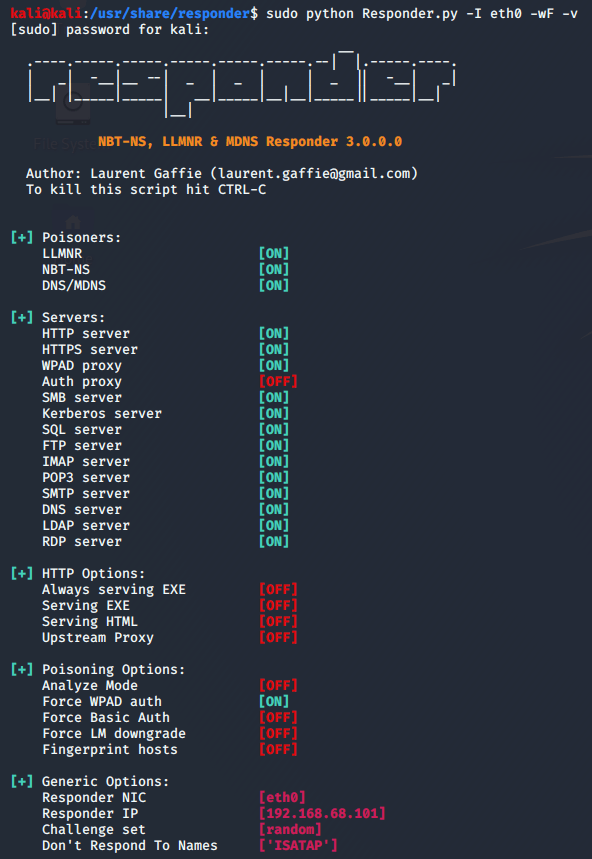
\includegraphics[width=0.75\linewidth]{responder.png}
    \caption{Enter Caption}
    \label{fig:placeholder}
\end{figure}

Here is how this attack scenario will plan out, but first, a quick overview of some DNS fundamentals you must understand. Name Resolution (abbreviated as NR) is a series of procedures conducted by a machine when it tries to retrieve another host's IP address by its hostname. On Windows machines, the procedure will roughly be as follows:
\begin{itemize}
    \item The hostname fileshare's IP address is required.
    \item The local host file will be checked for suitable records.
    \item If no records are found, our machine will move on to the local DNS cache, which archives recently resolved domain hostnames, both internal and external to the DNS server.
    \item No local DNS records found? A query will be sent to the configured DNS server.
    \item If all else fails, our machine will send a multicast query asking other machines on the same network leg for the fileshare's IP address.
\end{itemize}

As can be seen, the final fallback when resolving a hostname's IP address is using multicast NR. This is managed by three main protocols: NBT-NS (NetBIOS Name Service), LLMNR (Link-Local Multicast Name Resolution) and mDNS (multicast DNS).

The three protocols are used adjunctively for two main reasons: legacy support and compatibility. NBT-NS was created in the early 1980s and is somewhat in fitting with today's standards. As the protocol was falling out of favor, Windows machines started implementing NBT-NSs successor, LLMNR (still supporting NBT-NS for communications purposes with older machines). On the other hand, most Linux-based machines implemented mDNS instead. Eventually, with the release of Windows 11, Microsoft added support for mDNS as well to enhance overall compatibility with legacy systems left on the domain.

Before we go over this attack process, it is first necessary for us to understand exactly how attackers leverage the LLMNR, NBT-NS, and mDNS networking protocols to establish initial access. Once an attacker breaches an AD administered local network, they will want to gain as much privileges on the domain as quickly and as quietly as possible. LLMNR/NBT-NS poisoning is just one of the attack methods used to make this happen.

The LLMNR/NBT-NS Network Protocols
Link-Local Multicast Name Resolution (LLMNR) and NetBIOS Name Service (NBT-NS) are two name resolution services that Windows machines use to identify host addresses on a network when primary DNS resolution fails. LLMNR and NetBIOS are enabled by default on modern Windows computers.

When a user requests a named resource, the name of this resource needs to resolve to an IP address so that the user's computer knows where to send the network traffic. To resolve the name, the user's computer will take the following actions in order of priority:

\begin{enumerate}
    \item Check if the name resolves to the computer itself (localhost).
    \item Check to see if the name is in the cache or manually specified in the system's host file (\verb|C:\Windows\System32\drivers\etc\hosts|).
    \item Send a lookup request to the configured server.
    \item Broadcast an LLMNR name query to all machines on the local network.
    \item Broadcast an NBT-NS name query request to all machines on the local network.
\end{enumerate}

The LLMNR and NBT-NS queries will be sent to all other hosts on the local network, asking them to respond if they know the IP of the hostname being queried. Attackers can exploit this by responding with their own IP address to direct subsequent network traffic for the requested resource to their machine.

\subsection{How an LLMNR and NBT-NS Poisoning Attack Works}
LLMNR (Link-Local Multicast Name Resolution) and NBT-NS (NetBIOS Name Service) poisoning is a network attack technique that exploits how Windows systems attempt to resolve hostnames when DNS resolution fails.

When a Windows machine cannot find a hostname in DNS, it broadcasts queries using LLMNR or NBT-NS to all other machines on the local network, asking: \textit{"Do you know the IP address of this hostname?"} An attacker can intercept these broadcasts and reply with their own IP address, tricking the victim machine into sending sensitive authentication data.

In this example, we will walk through the process of performing an LLMNR/NBT-NS poisoning attack using \textbf{Responder},
 a popular penetration testing tool designed to capture authentication credentials from unsuspecting systems.

 \subsection{LLMNR/NBT-NS Poisoning Attack Chain}
 \subsubsection{Step 1: Starting the Poisoner}
 To begin the attack, we launch Responder with parameters telling it to listen on our chosen network interface (in this example, \texttt{eth0.} Responder will passively listen for LLMNR/NBT-NS queries, and, by default, also start multiple fake services such as Server Message Block (SMB), HyperText Transfer Protocol (HTTP), and File Transfer Protocol (FTP). These fake services will later receive authentication attempts from victims.

 \textbf{Command:}
 




\subsection{LLMNR, NBT-NS, and mDNS Query Process}

On our Windows 11 virtual machine, we mistyped a shared folder's name on purpose as \texttt{"filesahre"} instead of the correct way: \texttt{"fileshare,"} resulting in a series of mDNS, NBT-NS, and LLMNR queries. Notice that all of the queries are sent from our attacking machine to designated multicast addresses.

When attempting to access a shared folder on a Windows 11 virtual machine using a mistyped name like \textbackslash{}filesahre, the system will trigger a series of name resolution attempts, including LLMNR, NBT-NS, and mDNS. 

The process is as follows:
\begin{enumerate}
    \item \textbf{Local Resolution First:} The VM will initially try to resolve \texttt{fileshare} through its local DNS cache and configured DNS servers.
    \item \textbf{Fallback to Local Link Protocols:} If DNS fails, the system resorts to Link-Local Multicast Name Resolution (LLMNR) and NetBIOS Name Service (NBT-NS) to attempt resolution on the local network segment.
    \item \textbf{Multicast Queries:}
    \begin{enumerate}
        \item \textbf{LLMNR:} Sends multicast queries to IPv4 address \texttt{224.0.0.252} or IPv6 address \texttt{ff02::1:3} on UDP port 5355.
        \item \textbf{NBT-NS:} Uses broadcast or multicast messages over the local subnet, typically over UDP port 137.
        \item \textbf{mDNS:} Sends IP multicast UDP packets to IPv4 address \texttt{224.0.0.251} or IPv6 address \texttt{ff02::fb} on UDP port 5353.
    \end{enumerate}
\end{enumerate}


\textbf{Name Resolution }(abbreviated as \textbf{NR}), is a series of procedures conducted by a machine when it tries to retrieve another host’s IP address by its hostname. On Windows machines, the procedure will roughly be as follows:

1. The hostname \textit{fileshare’s }IP address is required.

2. The local hostfile will be checked for suitable records.

3. If no records are found, our machine will move on to the local DNS cache, which archives recently resolved domain hostnames, both internal and external to the DNS server.

4. No local DNS records found? A query will be sent to the configured DNS server.

5. If all else fails, our machine will send a multicast query asking other machines on the same network leg for the \textit{fileshare’s} IP address.

As can be seen, the final fallback when resolving a hostname’s IP address is using multicast NR. This is managed by three main protocols: \textbf{NBT-NS (NetBIOS Name Service), LLMNR (Link-Local Multicast Name Resolution), }and \textbf{mDNS (multicast DNS).}

The three protocols are used adjunctively for two main reasons: legacy support and compatibility and performance. NBT-NS was created in the early ‘80’s and is somewhat in fitting with today’s standards. As the protocol was falling out of favor, Windows machines started implementing NBT-NS’s successor, LLMNR (still supporting NBT-NS for communications purposes with older machines). On the other hand, most Linux-based machines implemented mDNS instead. Eventually with the release of Windows 11, Microsoft added support for mDNS as well to enhance overall compatibility with legacy systems left on the domain. 

Let’s see these protocols in action:

On our Windows 11 virtual machine, we mistyped a shared folder’s name on purpose (\textit{\textbackslash{}filesahre} instead of the correct way: \textbackslash{}\textit{fileshare}), resulting in a series of mDNS, NBT-NS, and LLMNR queries. Notice that all of the queries are sent from our attacking machine to designated multicast addresses.

\textit{\textbf{Figure X. }}\textit{Network capture of a Windows 11 machine trying to resolve an unknown hostname using multicast name resolution protocols}

You might be wondering why this is a problem. NBT-NS, LLMNR, and mDNS broadcast a query to the entire intranet, but no measures are taken to verify the integrity of the responses. This means that we can effectively exploit this mechanism by listening to such queries and spoofing the responses - tricking our mock user into trusting malicious server requests. Usually this trust will be used to steal their credentials.

The tool of choice for this scenario will be Python-based Responder on our Kali Linux machine.

\textbf{Common Abuse Cases}

There are many occasions in which a machine will resort to multicast NR, some of which are:

\textbf{Mistyping}

If a user mistypes the name of a legitimate host, usually no relevant host record will be found and the machine will resort to using multicast NR. This is a rather weak use case because we will have to wait for an error to appear on our mock victim user’s side.

\textbf{Misconfigurations}

False configurations on either the DNS server or our mock user’s client-side can lead to problems in NR and force the client to rely on multicast name queries for resolution.

\textbf{WPAD Protocol}

If a web browser is set to automatically detect proxy settings, it will use the WPAD protocol to discover the URL of a proxy configuration file. To discover this URL, WPAD will iterate through a series of potential URLs and hostnames - and with each false attempt, will expose itself to spoofing. Google Chrome and Firefox will not trigger this behavior, by default, but Internet Explorer and Bing will.

\textbf{Google Chrome}

When a single word string is typed into Chrome’s search bar, the application  needs a way to discern whether the string is indeed a legitimate URL or a search term. Chrome first treats the string as a search term and directs the user to its configured user engine, while simultaneously making sure the string is not a hostname by trying to resolve it. Furthermore, to prevent exposure to DNS hijacking attempts, Chrome will try to resolve several randomized hostnames upon startup to make sure they do not resolve - essentially guaranteeing some multicast NR action.

\textbf{Tips and Tricks}

In my experience, some tips that can better help you secure your network against Name Resolution (NR) attacks and protocol poisoning, as demonstrated with tools like Responder:

\textbf{1. Disable LLMNR and NBT-NS: }These legacy protocols are primary targets for NR poisoning attempts. By disabling them, you significantly reduce the attack surface making it harder for attackers to use this specific technique.

\textbf{2. Enable SMB Signing: }This prevents Man-in-the-Middle (MiTM) and relay attacks, protecting against unauthorized access to network resources.

\textbf{3. Use Host-based Firewalls: }Blocking multicast NR traffic at the host-level makes it harder for attackers to receive or inject spoofed responses.

\textbf{4. Monitor for unusual NR Traffic: }Keeping a continuous eye on network and host activities for suspicious NR-related traffic can help you quickly identify potential attacks before they have a chance to strike.

\textbf{5. Implement Strict DNS Configurations: }Ensuring proper DNS configurations prevents clients from falling back to using vulnerable multicast NR protocols, reducing exposure to spoofing attacks.

\textbf{Poisoning with Responder}

Responder is an open-source Python-based LLMNR/NBT-NS/mDNS poison acting into two stages: 

1. First, it will listen to multicast NR queries (LLMNR - UDP/5355, NBT-NS - UDP 137) and, under the right conditions, spoof a response - directing our victi to the machine on which it is running.

2. Once our mock vicctim will try and connect to our machine, Responder will then exploit the connection to steal credentails and other data.

In this specific scenario, we will use Responder to access credentials through SMB and WPAD authentication. We used a Kali Linux machine, which has this tool pre-installed and can be accessed under /usr/share/responder.

\textbf{Step 1: Setting Up}

This is our network setup:

\textit{Figure X. Demonstration network diagram, depicting the victim PC, attacker PC, and a file server named ‘fileshare.’}

Now, let’s see Responder’s arguments on our attacking machine (192.168.68.111):

\textit{\textbf{Figure X.}}\textit{ The Responder tool’s arguments (running on a Kali Linux virtual machine)}

We can see that WPAD capabilities are turned off by default, and to activate them we will add the flags -w and -F (to force the client to authenticate to us as part of the WPAD protocol). Coupled with the -I flag (to specify the interface to run on), and the -v flag (verbose mode), we will execute the following command:

kali@kali/user/share/responder\$ sudo python Responder.py -I etho0 -wF -v [sudo] password for kali:

\textit{Figure X. Responder’s enabled and disabled services and options, as displayed after app execution}

Now everyting is set up and Responder will now wait for any mutlicast NR queries to come in.

\textbf{Step 2: Attacking the Target}

\textbf{SMB Credential Access}

Remember our aformentioned mistype “\textit{||fileshare”}? This is how the same event looks on our attacking machine:

\textit{\textbf{Figure X. }}\textit{NR spoofing leading to SMB credentialed access, as seen on Responder’s log}

As seen in the introduction, several NBT-NS, LLMNR, and mDNS queries were broadcasted by our victim Windows 11 machine, indicating that the required hsot is supposed to be a file server. Responder will reply to file server queries via SMB and FTP by default. The victim ehten established a connection with our malicious SMB server and handed us its credentials.

Let’s visualize this process on Wireshark:

\textit{Figure X. NR spoofing leading to credentialed access, as seen on a Wireshark packet capture}

First our victim (192.168.62.101) sent multiple multicast NR queries using mDNS, NBT-NS (NBNS) and LLMNR. As seen in the second packet, Responder replied to the NBT-NS query claiming our machine (192.168.68.111) as \textit{filesahre:}

\textit{Figure X. Poisoned NBT-NS answer for fileshare (mistyped on purpose as ‘filesahre’)}

The victim then initiated an SMB connection and authenticated to our server, as seen in the last two packets. The username and password hash code were transferred and are now visible to us in plaintext form (“User: WINDEV2004EVAL\textbackslash{}User”). The full hash code is dispersed among several fields in both packets and can be gathered manually, but Responder automatically puts them together - outputting the complete hash code seen in the analyzed log.


For defenders, mitigating NTLM relaying should be a top priority. Disabling LLMNR and NBT-NS, enabling SMB signing across all systems, and monitoring for suspicious authentication patterns are effective defensive strategies to shut down this attack vector (and coupled with firewall rules and edge router ACLs) for good. The below figure illustrates the NTLM hash of an administrator credentialed information that was intercepted by the Responder tool.

 